\documentclass{../../td}
\usepackage{amsmath}
\usepackage{graphicx}
\usepackage{../../raccourcis}

\newcommand{\nom}{TD8 : Modulation avec récupération de porteuse}
\renewcommand{\nomentete}{UE431 - \nom}

\begin{document}

\titre{\nom}

\noindent A-1) Le spectre des signaux modulant et modulé bilatéral sont :\\
\begin{center}
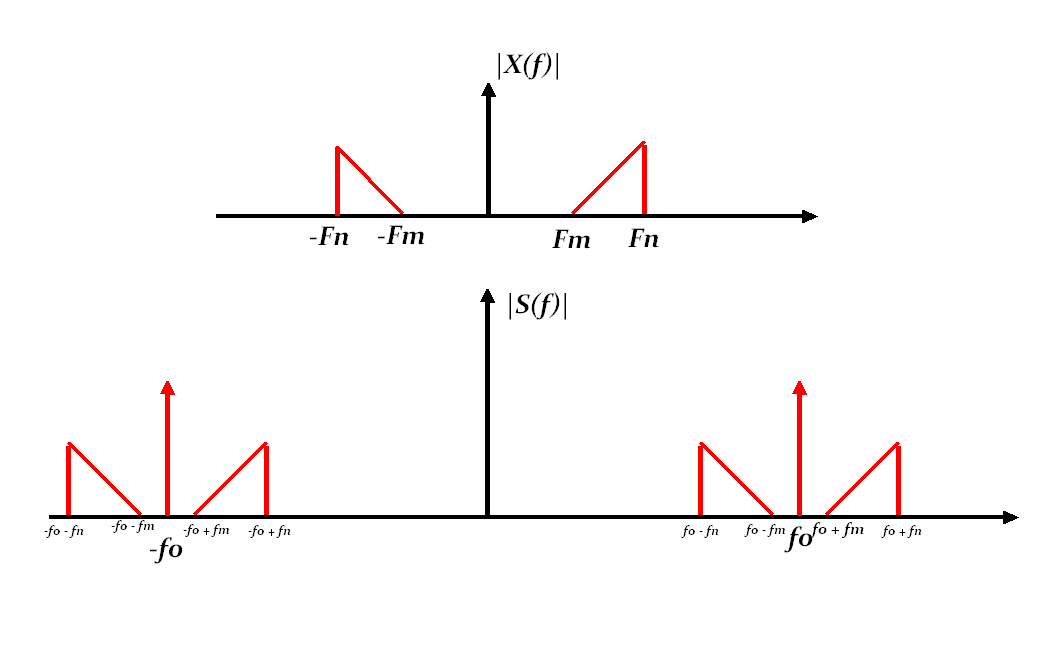
\includegraphics[scale=0.2]{TD8-1}
\end{center}
\noindent 2) Quel est le type de modulation?\\
\begin{align*}
s(t) &= kx(t)*p(t)+p(t)\\
&= p(t)[1+kx(t)]
\intertext{Or,}
m &= |kx(t)| = |kA_x| = \left | \frac{A_x}{V_0} \right | \geq 1
\end{align*}
On est donc en modulation d'amplitude à porteuse conservée avec surmodulation pour faciliter la récupération de la porteuse en réception.

\noindent B-Démolulation et réception
\noindent 1) On fait l'hypothèse que $\Phi_e(t) = 2\pi f_0t+\phi(t)$\\
Donc on a :
\[e(t) = A_eCos(\Phi_e(t)) = A_e cos(2\pi f_0t+\phi(t))\]
e(t) étant la sortie du VCO avec $f_i(t) =f_0 +a v(t)$ avec v(t) l'entrée du VCO\\

Exprimons $\phi(t)$ en fonction de $v(t)$ :\\
\begin{align*}
f_i(t) = \frac{1}{2\pi}\frac{d}{dt}\Phi_e(t) & \Rightarrow d\Phi_e(t) = 2\pi f_i(t)dt\\
& \Rightarrow \Phi_e(t) = 2\pi \int_0^t f_i(\tau) d\tau\\
& \Rightarrow \Phi_e(t) = 2\pi f_0 t + 2\pi a \int_0^t v(\tau) d\tau\\
& \Rightarrow \phi(t) = 2\pi a\int_0^tv(\tau)d\tau
\end{align*}
\bigbreak
\bigbreak

\noindent 2) Calculons u(t) en fonction de x(t),$f_0$ et $\phi(t)$ :
\begin{align*}
u(t) &= ks_r(t)e(t)\\
&= k A[1+kx(t)]cos(2\pi f_0t)A_e cos(2\pi f_0t + \phi(t))\\
&= kAA_e[1+kx(t)][\frac{1}{2}cos(4\pi f_0t + \phi(t))+\frac{cos(\phi(t))}{2}]
\end{align*}

\noindent 3) On veut seulement conserver $v(t) = kAA_e[1+kx(t)]\frac{cos(\phi(t)}{2}$ donc il faut :
\[F_n \leq f_{c1} << 2f_0\]

\noindent 4) Déterminons l'équation différentielle sur $\phi(t)$ où apparait x(t) :
\begin{align*}
\left \{ \begin{matrix}
f_i(t) = \frac{1}{2\pi}\frac{d}{dt}\Phi_e(t)\\
f_i(t) = f_0 + av(t)
\end{matrix} \right. &\Rightarrow  f_0 + av(t)=\frac{1}{2\pi}\frac{d}{dt}\Phi_e(t)\\
&\Rightarrow f_0 + av(t)=\frac{1}{2\pi}\frac{d}{dt}(2\pi f_0t + \phi(t))\\
&\Rightarrow f_0 + av(t)= f_0 + \frac{1}{2\pi}\frac{d\phi(t)}{dt}\\
&\Rightarrow \frac{1}{2\pi}\frac{d\phi(t)}{dt} = av(t) = akAA_e[1+kx(t)]\frac{cos(\phi(t))}{2}
\end{align*}

\noindent 5) Résolons l'équation différentielle en faisant apparaitre $\int x(t)dt$\\
Indication : $\int \frac{df}{cos(f)}=ln|tan(\frac{1}{2}+ \frac{\pi}{4})|$
D'après l'équation précédente on a :
\begin{align*}
\frac{df}{cos(f)} &= \pi akAA_e[1+kx(t)]dt
\intertext{d'où :}
ln|tan(\frac{\phi}{2}+ \frac{\pi}{4})| = \pi akAA_et + \pi a k^2AA_e\int_0^tx(\tau) d\tau + cst
\end{align*}

\noindent 6) Quelle est la valeur de $\phi_{\infty}$ ($\phi$ quand $t \rightarrow \infty$) si $x(t) = A_xcos(2\pi Ft)$ avec, $F_m<F<F_n$ ?\\

On prend l'exponentielle des deux membres de l'aquation précédente et il vient :
\[ |tan(\frac{\phi}{2}+ \frac{\pi}{4})| = e^{\pi akAA_et + \frac{\pi a k^2AA_eA_x}{2F}sin(2\pi Ft) + cst}\]
Or, l'exponentielle tend vers l'infini quand $t\rightarrow \infty$ donc la tangente tend vers l'infini ce qui correspond à :
\begin{align*}
\frac{\phi}{2}+ \frac{\pi}{4} = \pm \frac{\pi}{2} + 2n\pi \text{	 avec $n\in\mathbb{N}$} &\Rightarrow \phi_{infty} = \pm \pi -\frac{\pi}{2} + 4n\pi\\
&\Leftrightarrow \left \{ \begin{matrix}
\phi_{infty} = \frac{\pi}{2}+4n\pi\\
\phi_{infty} = -\frac{3\pi}{2}+4n\pi
\end{matrix} \right. \\
&\Leftrightarrow \phi_{infty} = \frac{\pi}{2} + 4n\pi
\end{align*}
\bigbreak
\bigbreak

\noindent 7) Le terme qui permet de connaitre $f_{\infty}$ est dû à la conservation de la porteuse (à l'émission).\\
En effet, il est responsable du terme $e^{\pi a k A A_e t}$ qui tend vers l'infini.
Le résultat $\phi_{\infty} = \frac{\pi}{2}$ serait le même quelque soit x(t).\\

\noindent 8) 
\begin{align*}
y(t) &= ks_r(t)*e(t)*\Phi(t)\\
&= Acos(2\pi f_0t)[1+kx(t)]cos(2\pi f_0t + \phi_{\infty} + \Phi)\\
&= \frac{A}{2}(cos(\phi_{\infty}+\Phi)+cos(4\pi f_0t) + \phi_{\infty}+\Phi))[1+kx(t)]
\end{align*}
\bigbreak
\bigbreak

\noindent 9) $F_m < 2 f_{c2} << 2f_0$ et $x(t) = \frac{kAA_e}{2}[1+kx(t)]$

\noindent 10) $\Phi_{opt}$ tel que $|cos(\phi_{\infty} - \Phi)| + \frac{Pi}{2}$
\end{document}
